\documentclass[11pt,twoside,a4paper]{article}
\usepackage{cite}
\usepackage[cm]{fullpage}
\usepackage{graphicx}
\usepackage{feynmp}
\usepackage{amsmath}
\usepackage{amssymb}
\DeclareGraphicsRule{*}{mps}{*}{}
\usepackage{caption}
\usepackage{subcaption}
\usepackage{slashed}
\usepackage[utf8]{inputenc}


\begin{document}
\begin{fmffile}{feynmandiags}

\title{Searches for Higgs boson decays to invisible final states at the Compact Muon Solenoid}
\author{Patrick Dunne \\ Supervisors: David Colling, Gavin Davies}
\maketitle


\renewcommand{\abstractname}{\vspace{-\baselineskip}}
\begin{abstract}
%!!REVIEW AT END
  An overview of searches for invisible decays of Higgs bosons at the Compact Muon Solenoid (CMS) at the Large Hadron Collider (LHC) is presented. A particular emphasis is placed on the search for invisible Higgs boson final states in the vector boson fusion (VBF) production channel and the combination of the results of this search with those from two other searches in the Z boson associated production channel. By combining the results from all the search channels an observed (expected) upper limit on the invisible branching fraction of a 125 GeV Higgs boson of 0.58 (0.44) is placed at the 95\% confidence level, assuming standard model Higgs boson cross sections and acceptances.
\end{abstract}


\section{Theoretical Background}
\label{theory}
The Standard Model (SM) of particle physics is one of the most successful physical theories devised, and one of its cornerstones is electroweak unification \cite{glashow,weinberg,salam}. Electroweak unification proposes that the Lagrangian has an SU(2)xU(1) symmetry and local gauge invariance with four gauge bosons, the photon ($\gamma$) and the $W$ and $Z$ bosons. It was already know that massive exchange particles would be required to explain the short range of the weak force, and indeed the new particles predicted by the theory, the $W$ and $Z$ bosons, were observed at the UA1 and UA2 experiments in 1983 \cite{wdiscovery,zdiscovery}, with masses of 80.4 GeV and 91.2 GeV, respectively. Unfortunately the symmetry of the Lagrangian is ruined by vector boson mass terms, so a different mechanism is required to give mass to the particles we observe.

The Higgs mechanism provides a solution to this problem by adding a complex scalar field with a non-zero vacuum expectation value, the Higgs field, to the Lagrangian that couples to the gauge bosons \cite{englertbrout,higgs1,higgs2,guralniketc,higgs3,kibble}. While the Lagrangian term itself respects the symmetry described above, the ground state does not; this is called spontaneous symmetry breaking. The gauge bosons coupling to a field with a non-zero vacuum expectation accounts for their mass, and we are left with the prediction of a new massive scalar boson, the Higgs boson. A Higgs boson has recently been discovered by the ATLAS and CMS \cite{cmsdiscovery,atlasdiscovery} experiments at CERN.

However, despite all current measurements of the properties of this Higgs boson being consistent with the SM, the precision of these measurements is not sufficient to determine whether or not it is a SM Higgs boson. Furthermore, despite additional SM-like Higgs bosons being excluded across a wide mass range, exotically decaying Higgs bosons, predicted by many beyond the SM theories \cite{higgworkgroup2001}, are not ruled out. The motivation for searches for invisibly decaying Higgs bosons is therefore strong.


\begin{figure}
  \centering
  \raisebox{-0.5\height}{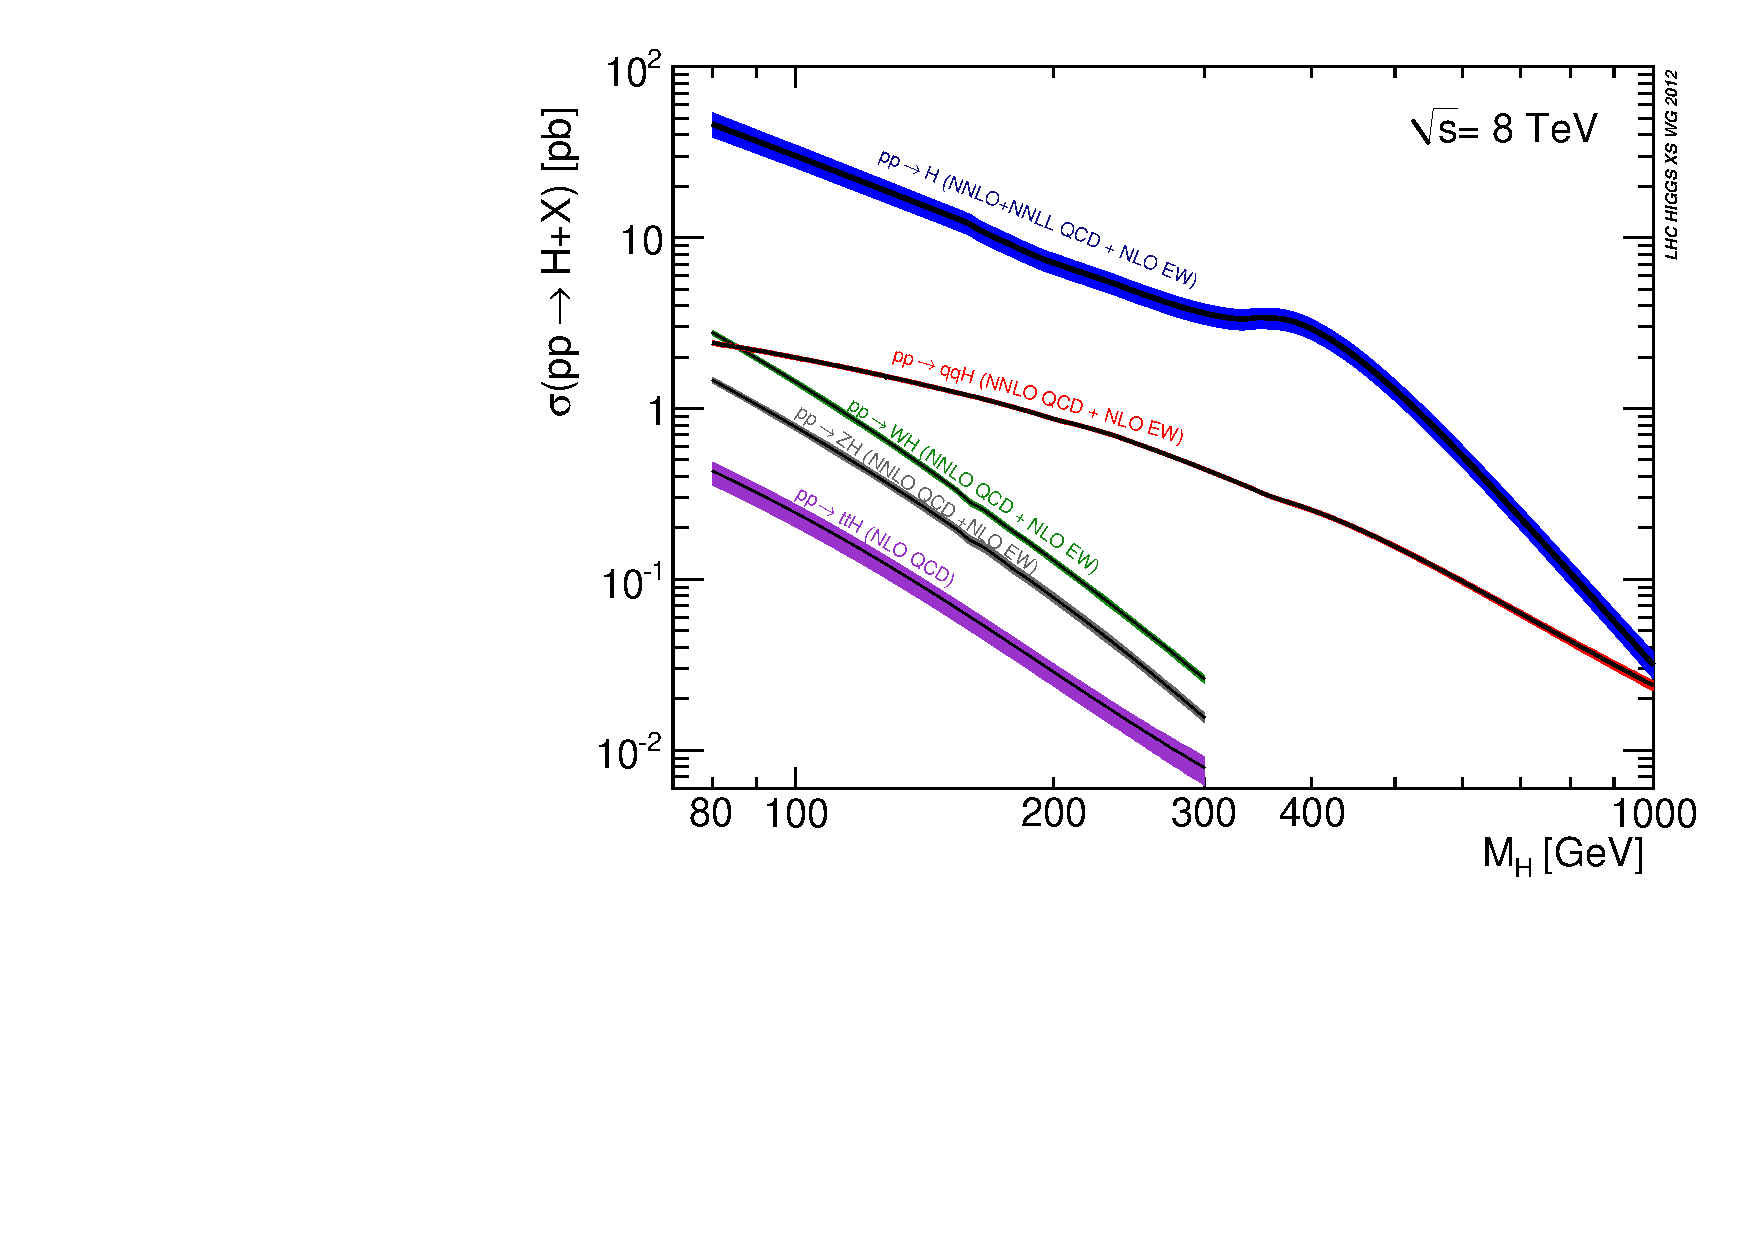
\includegraphics[width=0.49\textwidth]{Images/Higgs_XS_8TeV_lx.pdf}}
%  \raisebox{-0.5\height}{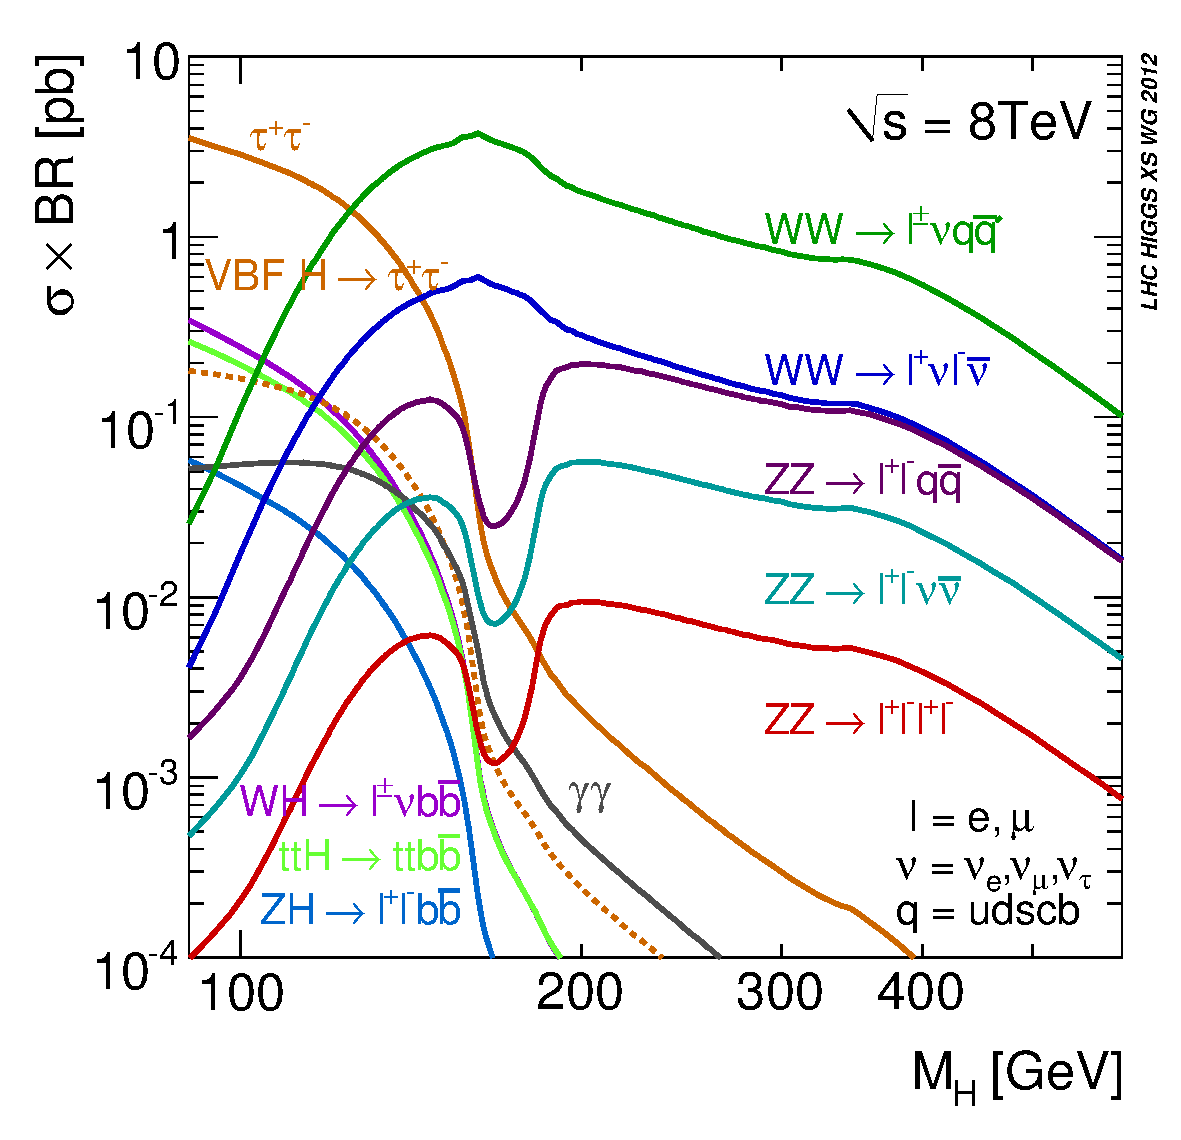
\includegraphics[width=0.49\textwidth]{Images/XSBR_8TeV_SM.pdf}}
  \caption{The cross-section for SM Higgs boson production mechanisms is shown, $pp \rightarrow H$ is gluon fusion, $pp \rightarrow qqH$ is VBF and the remaining three are associated production with $W$, $Z$ and $t\bar{t}$. From \cite{lhchxswg}}.
  \label{higgbrfig}
\end{figure}


\begin{figure}
  \centering
  \begin{subfigure}{0.24\textwidth}
    \centering
    %ggf 
    \begin{fmfgraph*}(75,100)
      \fmfleft{i0,i1,i2,i3,i4,i5}
      \fmfright{o1}
      \fmf{gluon}{i1,v1}
      \fmf{gluon}{i4,v2}
      \fmf{fermion,tension=0}{v1,v2}
      \fmf{fermion,tension=2/3}{v2,v3,v1}
      \fmf{dashes}{v3,o1}
      \fmflabel{$g$}{i1}
      \fmflabel{$g$}{i4}
      \fmflabel{$H$}{o1}
    \end{fmfgraph*}
    \caption{}
  \end{subfigure}
  \begin{subfigure}{0.24\textwidth}
    \centering
    %vbf                                                                                                   
    \begin{fmfgraph*}(75,100)
      \fmfleft{i1,i2}
      \fmfright{o1,o2,o3}
      \fmf{fermion}{i1,v1,o1}
      \fmf{fermion}{i2,v2,o3}
      \fmf{photon,label=$W,,Z$}{v1,v3}
      \fmf{photon,label=$W,,Z$}{v2,v3}
      \fmf{dashes}{v3,o2}
      \fmflabel{$q$}{i1}
      \fmflabel{$q$}{i2}
      \fmflabel{$q$}{o1}
      \fmflabel{$q$}{o3}
      \fmflabel{$H$}{o2}
    \end{fmfgraph*}
    \caption{}
  \end{subfigure}
  \begin{subfigure}{0.24\textwidth}
    \centering
    %Higgstrahlung
    \begin{fmfgraph*}(75,100)
      \fmfleft{i1,i2}
      \fmfright{o1,o2}
      \fmf{fermion}{i1,v1}
      \fmf{fermion}{v1,i2}
      \fmf{photon,label=$W,,Z$}{v1,v2}
      \fmf{photon}{v2,o1}
      \fmf{dashes}{v2,o2}
      \fmflabel{$q$}{i1}
      \fmflabel{$\bar{q}$}{i2}
      \fmflabel{$W,Z$}{o1}
      \fmflabel{$H$}{o2}
    \end{fmfgraph*}
    \caption{}
  \end{subfigure}
  \begin{subfigure}{0.24\textwidth}
    \centering
    %ttH                                                                                                    
    \begin{fmfgraph*}(75,100)
      \fmfleft{i0,i1,i4,i5,i6,i2,i3}
      \fmfright{o0,o1,o2,o3,o4}
      \fmf{gluon,tension=3/2}{i1,v1}
      \fmf{gluon,tension=3/2}{i2,v2}
      \fmf{fermion}{o1,v1,v3,v2,o3}
      \fmf{dashes,tension=3/2}{v3,o2}
      \fmflabel{$g$}{i1}
      \fmflabel{$g$}{i2}
      \fmflabel{$\bar{t}$}{o1}
      \fmflabel{$t$}{o3}
      \fmflabel{$H$}{o2}
    \end{fmfgraph*}
    \caption{}
  \end{subfigure}
  \caption{The Feynman diagrams for the Higgs production mechanisms at CMS are shown: a) gluon fusion, b) vector boson fusion, c) $W$/$Z$ associated production and d) $t\bar{t}$ associated production.}
  \label{higgprodfig}
\end{figure}

\section{Search Channels}
\label{proddec}
As can be seen in Fig.~\ref{higgbrfig} the SM Higgs boson production mechanism with the highest cross-section at the LHC is gluon fusion (ggF) which proceeds through a quark loop as shown in Fig.~\ref{higgprodfig}a. However, a ggF produced Higgs boson that decayed invisibly would leave no signature in the detector. It is only in channels where the Higgs is produced recoiling against a visible system that invisible searches can be carried out.

After ggF the next highest production cross-section is for vector boson fusion (VBF), which occurs through the Feynman diagram shown in Fig.~\ref{higgprodfig}b. VBF produced Higgs bosons recoil against two quarks, so this channel can be used for invisible searches. VBF production also has the advantage that the two quarks are produced with a large pseudorapidity (defined in Sec. \ref{cmslhc}) gap between them, which can be used as a signature to trigger on \cite{zeppenfeld}.

After VBF is associated production with a Z boson (ZH) as shown in fig. \ref{higgprodfig}c, which can also be used for searches for invisible decays by studying the decay products of the Z boson. Furthermore, when the Z boson decays leptonically this channel has the advantage of providing a very clean signature with much lower backgrounds than VBF.

Finally there is associated production, with a $t\bar{t}$ pair through the diagram in fig. \ref{higgprodfig}d. Despite the Higgs recoiling against the visible $t\bar{t}$ system the very low cross-section for this process makes it impossible to carry out a search for invisible decays in this channel with the currently available amounts of data.

This report will describe searches performed at the CMS experiment, with an emphasis on the VBF channel, and the combination of the VBF result with those from two searches in the ZH production mode, one where the Z boson decays to two leptons, and the other where it decays to two b quarks.


\section{CMS and the LHC}
\label{cmslhc}
The LHC is a proton proton collider situated at CERN near Geneva with nominal centre of mass energy ($\sqrt{s}$) of 14 TeV. It ran in 2010 and 2011 at $\sqrt{s}$ = 7 TeV, and again in 2012 at $\sqrt{s}$ = 8 TeV. The CMS detector is one of the two general purpose detectors at the LHC, the other being ATLAS. From the inside out it comprises: a central silicon detector for vertex location and tracking, an electromagnetic calorimeter (ECAL), a hadronic calorimeter (HCAL), a superconducting magnet to bend particle tracks for momentum measurement and a muon system situated in the magnet return yoke\cite{cmstdr}.

The co-ordinate system used by CMS is right-handed with the x-axis pointing to the centre of the LHC ring, the y-axis pointing vertically upwards and the z axis along the beam-line. The spherical polar co-ordinates $\theta$ and $\phi$ take their normal definitions. CMS also uses the pseudorapidity variable, $\eta$, which is defined as
\begin{equation}\label{pseudorap}
  \eta = -\ln\tan(\frac{\theta}{2}).
\end{equation}

All the subdetectors cover the full $2\pi$ range in $\phi$, except for small regions blocked by services such as power cabling and cooling. The pseudorapidity ranges of the subdetectors vary and are described in Table \ref{rapranges}.

The tracker consists of an inner pixel detector and an outer silicon strip detector. Both the pixel and strip detectors are split into a barrel section and endcaps. The pixel detector has a resolution  of 15-20 $\mu$m in r-$\phi$ and z giving vertex resolutions of 30-40 $\mu$m in the longitudinal direction, while the strip detector has a resolution in the range 23-52 $\mu$m in r-$\phi$ and 230-530 $\mu$m in z \cite{cmstdr}. This high accuracy is necessary to discriminate between tracks from pileup (particles from interactions other than the interaction of interest) and the collision of interest; it also improves the energy resolution of objects reconstructed by matching calorimeter deposits to tracks. The tracker determines particle momentum from the curvature of tracks, achieving a resolution of 1-2\% for 100 GeV particles with $\eta<1.6$ \cite{cmstdr}.

The ECAL is a homogeneous PbWO$_{4}$ scintillating calorimeter which is split into a barrel section and an endcap section. Its energy resolution is energy dependent and is well described by:
\begin{equation}\label{sigmaE}
  \frac{\sigma}{E} = \frac{\alpha}{\sqrt{E}}\sqrt{\rm{GeV}} \oplus \frac{\beta}{E}\rm{GeV} \oplus \delta\,.
\end{equation}
with $\alpha$ = 2.8\%, $\beta$ = 0.12 and $\delta$ = 0.3\% \cite{cmstdr}. The ECAL energy resolution is important in determining the accuracy of any missing energy calculation, making it key to Higgs to invisible searches. The sensitivity of the Higgs to $\gamma\gamma$ channel is also very dependent on good ECAL energy resolution.

\begin{table}
  \centering
\begin{tabular}{|l|c|}
    \hline
    Subdetector & Pseudorapidity Range \\
    \hline
    Tracker & $|\eta|<2.5$ \\
    ECAL & $|\eta|<3.0$\\
    HCAL (excluding forward region) & $|\eta|<3.0$ \\
    Forward HCAL & $3.0<|\eta|<5.0$ \\
    Muon system & $|\eta|<2.4$ \\
    \hline
\end{tabular}
\caption{The pseudorapidity ranges of the sub-detectors of the CMS experiment}
\label{rapranges}
\end{table}


The HCAL is made up of a barrel region and endcaps. The barrel and endcaps are sampling calorimeters composed of interleaved brass and plastic scintillator. The forward HCAL is a steel and Cherenkov emitting quartz fibre sampling calorimeter. The energy resolution of the HCAL and ECAL combined, which is the figure most important for missing energy determination, is well described by Eq. \ref{sigmaE} with $\alpha$=1.21 GeV$^{1/2}$, $\beta$=0.095 and $\delta$=0 \cite{hcalres}. The forward HCAL is particularly important for the Higgs to invisible search, and any other VBF processes, because the large pseudorapidity gap expected means that 80\% of VBF events with a pseudorapidity gap of at least 4.4 will have at least one jet in the forward HCAL \cite{higgworkgroup2001}.

The muon system is situated in the return yoke of the superconducting magnet and consists of a drift tube system in the barrel section of the detector, a cathode strip chamber system in the endcap and a resitive plate chamber system both in the endcaps and the barrel. Combined with inner tracker information the muon system gives a momentum resolution of $\delta p_{T}$/$p_{T}$ between 0.01 and 0.1 for muons with $p_{T}$ between 10 and 1000 GeV.

To date an integrated luminosity of 5.6 fb$^{-1}$ has been recorded by CMS at $\sqrt{s}$ = 7 TeV, and 21.8 fb$^{-1}$ have been collected at $\sqrt{s}$ = 8 TeV. However, the rate of collisions at the LHC is too great for CMS to record every detected event; a triggering process is therefore necessary to select the most interesting events for recording. At CMS the trigger consists of the level one trigger which is hardware based, and the higher level trigger (``HLT'') which is software based \cite{cmstdr}.

For the 2012 run it was realised that whilst it is only possible to process events at a rate of 700 Hz an extra 1000 Hz could be stored to tape for later processing \cite{parkeddata}. This extra data is referred to as ``parked data'' and is of particular relevance to the Higgs to Invisible search discussed in Sec. \ref{htoinv}.

\section{VBF Higgs to invisible}
\label{htoinv}
In several beyond the SM theories the Higgs boson is expected to have a significant branching ratio for decays to particles that would be invisible to the CMS detector \cite{higgworkgroup2001}. The VBF channel has been shown to be the most sensitive production channel to decays to invisible final states \cite {bds}; this is because of its high cross-section compared to the associated production channels and its more distinctive topology compared to ggF as seen in Section \ref{proddec}.

\subsection{Event Selection}
The strategy that has been used is to select events with the distinctive VBF Higgs production topology to tag Higgs events and then search for missing energy consistent with an invisibly decaying Higgs boson.In addition to the gap in pseudorapidity, jets produced in VBF processes are expected to be in opposite halves of the detector. Furthermore, QCD backgrounds can be significantly suppressed whilst retaining high signal efficiency by requiring a high dijet invariant mass \cite{zeppenfeld}. CMS has a dedicated trigger for this analysis which requires two jets and the following other conditions:
\begin{equation}E_{T_{j_{1,2}}} >40\,\rm{GeV}, \eta_{j_{1}} \cdot \eta_{j_{2}} < 0, \Delta\eta_{jj} > 3.5, M_{jj} > 800\,\rm{GeV}, \slashed{E}_{T} > 65\,\rm{GeV},
\end {equation}
 where $\slashed{E}_{T}$ is the missing transverse energy. Other than the missing $E_{T}$ trigger, which is specific to invisible decays, these are generic cuts for VBF analyses \cite{hig1330}.

Even after the trigger selection for the VBF topology and missing energy, there are still significant backgrounds to a Higgs to invisible search. Both $Z$ + jets and $W$ + jets where the leptons are missed have missing energy and can occur via VBF and thus also have the same pseudorapidity gap. Further backgrounds are expected from mismeasured QCD events which give fake missing energy. $W$ + jets and $Z$ + jets also occur via QCD and produce further backgrounds \cite{bds}. Further offline cuts are made and take the form of:
\begin{equation}E_{T_{j_{1,2}}} > 50 \,\rm{GeV}, \eta_{j_{1}} \cdot \eta_{j_{2}} < 0, |\eta_{j_{1,2}}| < 4.7, \Delta\eta_{jj} > 4.2, M_{jj} > 1100 \,\rm{GeV}, \slashed{E}_{T} > 130 \,\rm{GeV},\Delta\phi_{jj}<1.0.
\end{equation}
We also apply a Central Jet Veto (CJV), which involves vetoing any event where there is an addtional jet with $p_{T}$ greater than 30 GeV between the two VBF jets, and a lepton veto, removing any events with an electron or muon with $p_{T}>10$ GeV. The CJV, lepton veto and $\Delta\phi_{jj}$ cut values are selected to reduce backgrounds, whilst the values of the remaining cuts are chosen so that the effect of trigger inefficiencies is small \cite{hig1330}.

After the full selection 210 signal events are expected for a 125 GeV Higgs boson with the SM VBF production cross-section that decays entirely to invisible final states. For a fully invisible 125 GeV Higgs boson with SM production cross-sections we would also expect 14 events in the signal region from ggF production.

\subsection{Background Estimation}
\label{bkgest}
Whilst the cuts applied in this analysis do significantly reduce the presence of backgrounds, they also mean that the signal region is in a region of phase space which is not well modelled by Monte Carlo simulation (MC). Remaining major backgrounds must therefore be estimated from data control regions. The assumption of the methods used is that whilst the overall MC normalisation cannot be trusted, the shapes of the MC are reliable. The ratio of the number of events in the signal region to that in the control region can therefore be taken from MC, and used in conjunction with the data yield in the control region to give an estimate of the remaining background.

For the $W$ + jets backgrounds the control region used is to replace the lepton veto with a lepton requirement, and in the case where the $W$ decays to a muon to recalculate the missing $E_{T}$ ignoring the muon. The following formula is then used to give an estimate of the remaining background:
\begin{equation}
  N_{S}^{Data}=\frac{N_{S}^{MC}}{N_{C}^{MC}}\cdot \left( N_{C}^{Data} - N_{C}^{Bkg} \right)
\end{equation}
where $N_{S}^{Data}$ is the remaining background in the signal region, $N_{S/C}^{MC}$ is the MC yield in the signal/control region, $N_{C}^{Data}$ is the data yield in the control region and $N_{C}^{Bkg}$ is the number of events in the control region from other minor backgrounds, such as diboson and top quark production, in the control region estimated from MC.

For the $Z$ + jets background the control region used is the region where the muon veto is replaced with a requirement of two muons whose invariant mass is compatible with the $Z$ mass peak, and the missing $E_{T}$ is recalculated ignoring the muons. The formula used in this case is slightly more complicated as dimuon production in association with jets can procede through a virtual photon as well as via a $Z$, and so has a different cross-section to the case where the $Z$ decays invisibly, this must therefore be corrected for. The formula used is as follows:
\begin{equation}
  N_{S}^{Data}=\frac{N_{S}^{MC}}{N_{C}^{MC}}\cdot \frac{\sigma\left(Z\rightarrow\nu\nu\right)}{\sigma\left(Z/\gamma^{*}\rightarrow\mu\mu\right)} \cdot \left( N_{C}^{Data} - N_{C}^{Bkg} \right)
\end{equation}

Due to limited statistics the QCD background is estimated using an ABCD method, the formula used is as follows:
\begin{equation}
  N_{S}^{QCD}=\frac{N_{B}^{Data}\cdot N_{C}^{Data}}{N_{A}^{Data}},
\end{equation}
where $N_{S}^{QCD}$ is the estimate of the remaining QCD background and $N_{A/B/C}^{Data}$ are the number of events in data in the regions A, B and C which are defined as follows:
\begin{itemize}
\item Region A: Events failing the CJV and missing $E_{T}$ cuts, but passing the full remaining selection
\item Region B: Events failing the CJV cut, but passing the full remaining selection
\item Region C: Events failing the missing $E_{T}$ cut, but passing the full remaining selection
\end{itemize}
This method relies on the assumption that the missing $E_{T}$ and CJV are uncorrelated, the missing $E_{T}$ distribution in the regions passing and failing the CJV has been checked, and a conservative 40\% systematic uncertainty is assigned to account for the maximum difference between the two distributions \cite{hig1330}.

Remaining minor backgrounds for top quark pairs, single tops and diboson events are estimated from MC. As these backgrounds contribute a very small amount to the overall number of events in the signal region the large uncertainties due to lack of confidence in the overall MC normalisation is considered acceptable.

The results of the above background methods are summarised in Table \ref{restable}.

\begin{table}
  \centering
\begin{tabular}{|l|c|}
    \hline
    Process & Event yields \\
    \hline
    \hline
    $Z(\nu\nu)+$jets & $ 99 \pm 29 (stat.) 25 \pm (syst.)$\\
    $W(\mu\nu)+$jets & $ 67 \pm 5 (stat.) 16 \pm (syst.)$\\
    $W(e\nu)+$jets & $63 \pm 9 (stat.) \pm 18 (syst.)$\\
    $W(\tau_{h}\nu)+$jets & $53 \pm 18 (stat.) \pm 18 (syst.)$\\
    QCD multijet & $31 \pm 2 (stat.) \pm 23 (syst.)$\\
    Sum ($t\bar{t}$, single top quark, VV, DY) & $20.0 \pm 8.2 (syst.)$ \\
    \hline
    Total background & $332 \pm 36 (stat.) \pm 46 (syst.)$ \\
    VBF H(inv.) & $210 \pm 30 (syst.)$\\
    ggF H(inv.) & $14 \pm 11 (syst.)$\\
    Observed & 390\\
    \hline
    S/B(\%) & 70\\
    \hline
\end{tabular}
\caption{ Summary of the estimated number of background and signal events, together with the observed yield, in the VBF search signal region. The signal yields are given for $m_{H}=125$ GeV and 100\% invisible branching fraction. Taken from \cite{hig1330}}
\label{restable}
\end{table}

\subsection{Systematic Uncertainties}
%!!LIMIT PLOTS, DISCUSS SYSTEMATICS
The dominant uncertainties in this analysis come from statistical uncertainties in the control regions and MC samples used for background estimation. After these effects the next most important source of systematic errors are the jet and unclustered energy scale and resolution uncertainties. An estimate of the size of these uncertainties is made by varying the energy scale and resolution of the jets and unclustered energy up and down by one standard deviation and repeating the analysis. Further uncertainties come from the differences seen between the met distribution passing and failing the CJV as described in section \ref{bkgest}, uncertainties in the electron and muon isolation efficiencies and uncertainties in the cross-sections, taken from CMS analyses, of the minor backgrounds. \cite{hig1330}

In addition to experimental uncertainties we also consider theoretical systematics arising from parton density function (PDF) uncertainties and factorisation and renormalisation scale uncertainties. A further theoretical uncertainty that we consider is the error in modelling of the ggF production in MC, this is estimated by comparing different MC generators, and although the resulting uncertainty is large the effect on the final result is small as the ggF yield is minimal.

The size of the above uncertainties relative to the total background and signal yield is summarised in table \ref{systtab}.

\begin{table}
  \centering
\begin{tabular}{|l|c|c|}
    \hline
    Source & Total Background & Signal \\
    \hline
    \hline
    Control region statistics & 11\% &  -\\
    MC statistics & 11\% &  4\%\\
    Jet/missing $E_{T}$ energy scale/resolution & 7\% &  13\%\\
    QCD background estimation & 4\% &  -\\
    Lepton efficieny & 2\% &  -\\
    Tau ID efficiency & 1\% & -\\
    Luminosity & 0.2\% &  2.6\%\\
    Cross sections & 0.5-1\% &  -\\
    PDFs & - &  5\%\\
    Factorization/renormalization scale & - &  4\%\\
    Gluon fusion signal modelling & - &  4\%\\
    
    \hline
\end{tabular}
\caption{Summary of the systematic uncertainties in the total background and signal yields in the VBF channel. All uncertainties affect the normalization of the yield, and are quoted with respect to the total background or signal estimate. The signal uncertainties are given for $m_{H}=125$ GeV and 100\% invisible branching fraction. Taken from \cite{hig1330}}
\label{systtab}
\end{table}

\section{Limits and Combination of search channels}
\label{combs}

%!!BELOW MAYBE REPLACE WITH REFERENCE
\subsection{Limit setting method}
A general methodology for placing limits has been developed by ATLAS and CMS which is described in detail in refs. \cite{lhccomb1,comb2011} and is summarised below as it appears in ref. \cite{hcpcomb2012}.

The CL$_{s}$ statistic is used, which is a function of the profile likelihood ratio, q$_{\mu}$, defined as:
\begin{equation}
  q_{\mu} = -2 \ln\frac{\mathcal{L}(obs|\mu \cdot s + b,\hat{\theta}_{\mu})}{\mathcal{L}(obs|\hat{\mu} \cdot s + b,\hat{\theta})}\,,
\end{equation}
where s is the SM expected Higgs signal and b is the background. $\mu$ is a signal strength modifier which is 1 for a SM Higgs boson and 0 for the background only case. $\theta$ are nuisance parameters, such as systematic errors, which include the errors and any correlations between them. $\hat{\mu}$ and $\hat{\theta}$ are the values of $\theta$ and $\mu$ where the likelihood, $\mathcal{L}$, is maximised, and $\hat{\theta}_{\mu}$ is the $\theta$ that maximises the likelihood for a given $\mu$. The profile likelihood ratio therefore describes how likely a given signal strength is compared to the most likely signal strength.

The definition of CL$_{s}$ is
\begin{equation}
  CL_{s} = \frac{P(q_{\mu}\geqslant q_{\mu}^{obs} | \mu \cdot s + b)}{P(q_{\mu}\geqslant q_{\mu}^{obs}|b)}\,,
\end{equation}
Where the method of the determining probability, $P$ ,varies. The region in which a signal strength $\mu \cdot s$ is excluded with $1 - \alpha$ confidence is then the region for which CL$_{s}$ is less than or equal to $\alpha$ i.e. when the background hypothesis is $1/\alpha$ times more likely than the signal hypothesis we exclude the signal hypothesis with $1 - \alpha$ confidence.

%!!SIGNAL YIELD INTERPOLATION INC PLOT


\subsection{Other search channels}
%!!BRIEF DISCUSSION OF OTHER CHANNELS
%!!CORRELATION OF NUISANCES

\subsection{Results}
%!!GIVE THE LIMIT NUMBERS

\begin{figure}
  \centering
  \raisebox{-0.5\height}{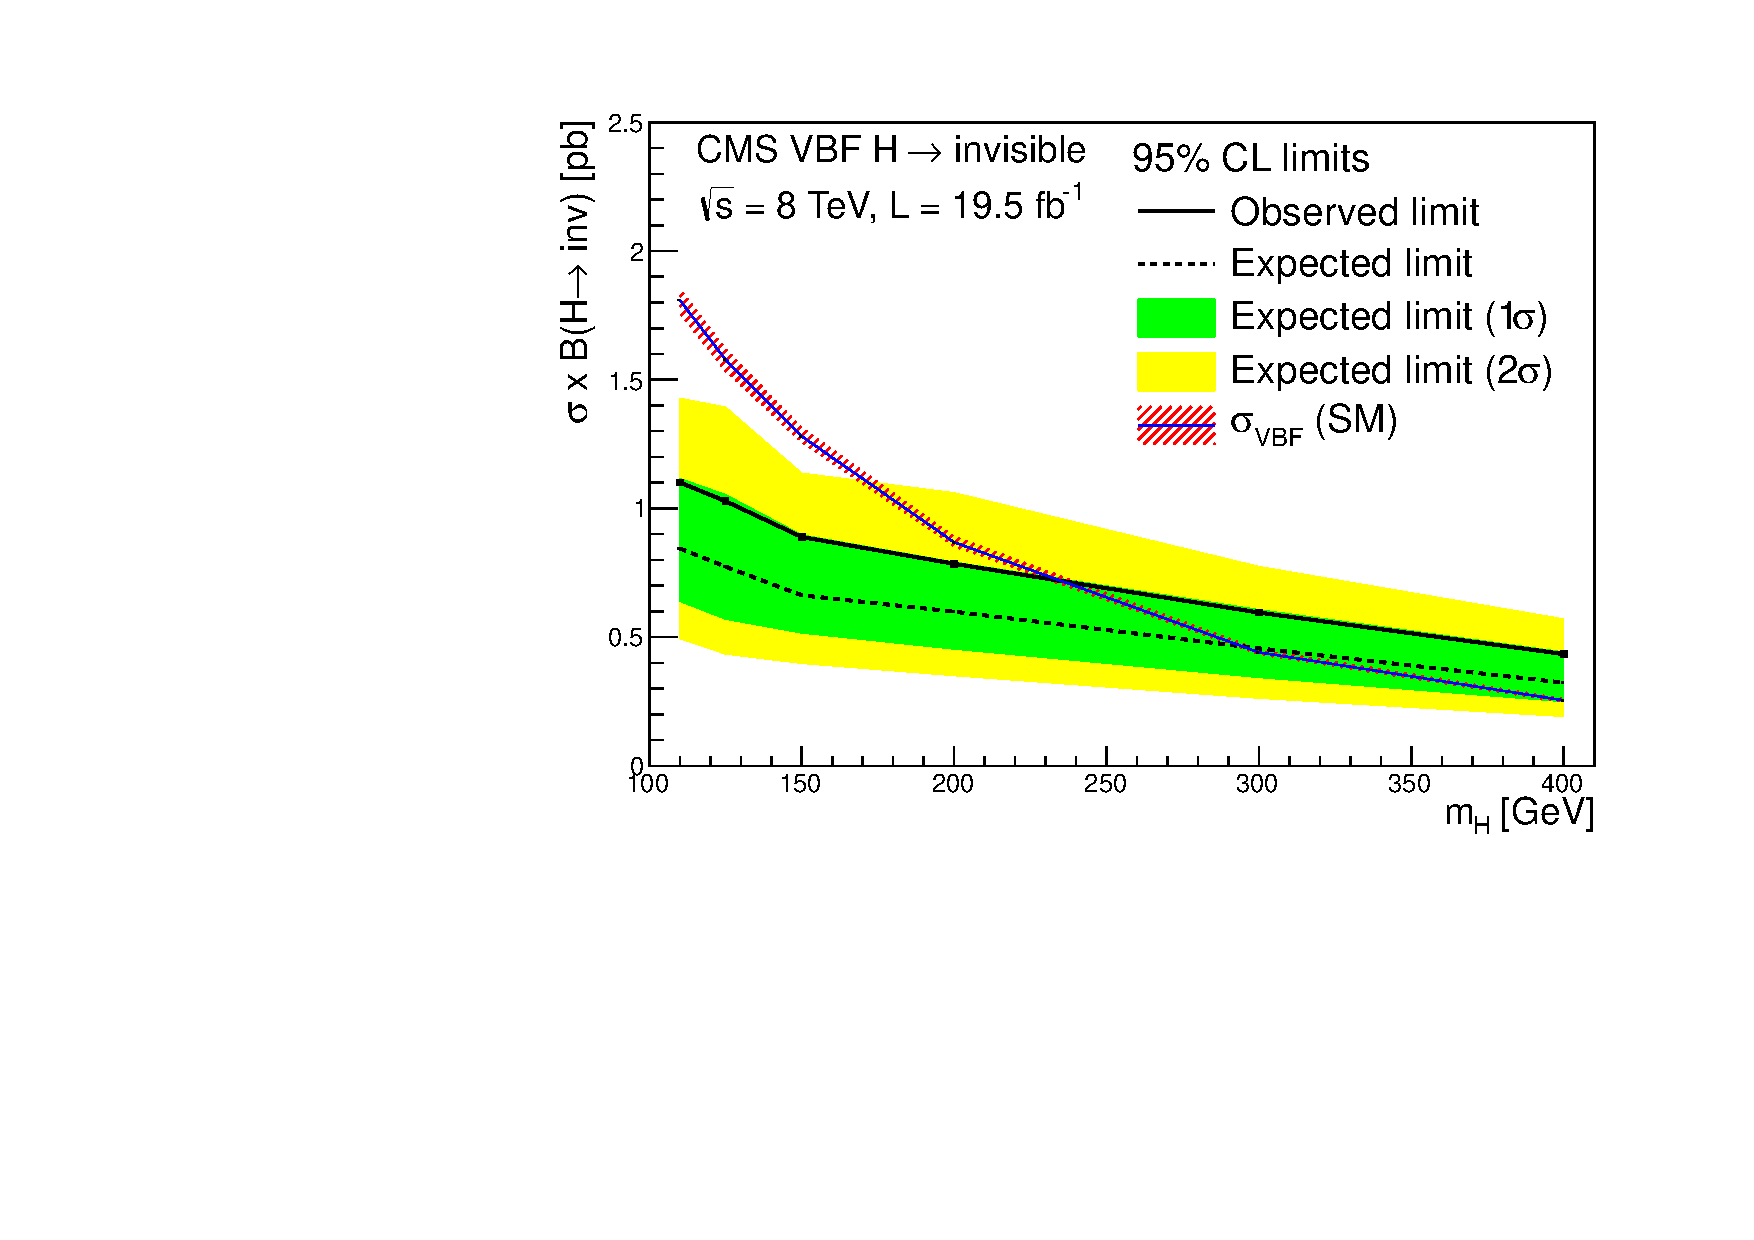
\includegraphics[width=0.49\textwidth]{Images/VBF-XSLimit.pdf}}
  \raisebox{-0.5\height}{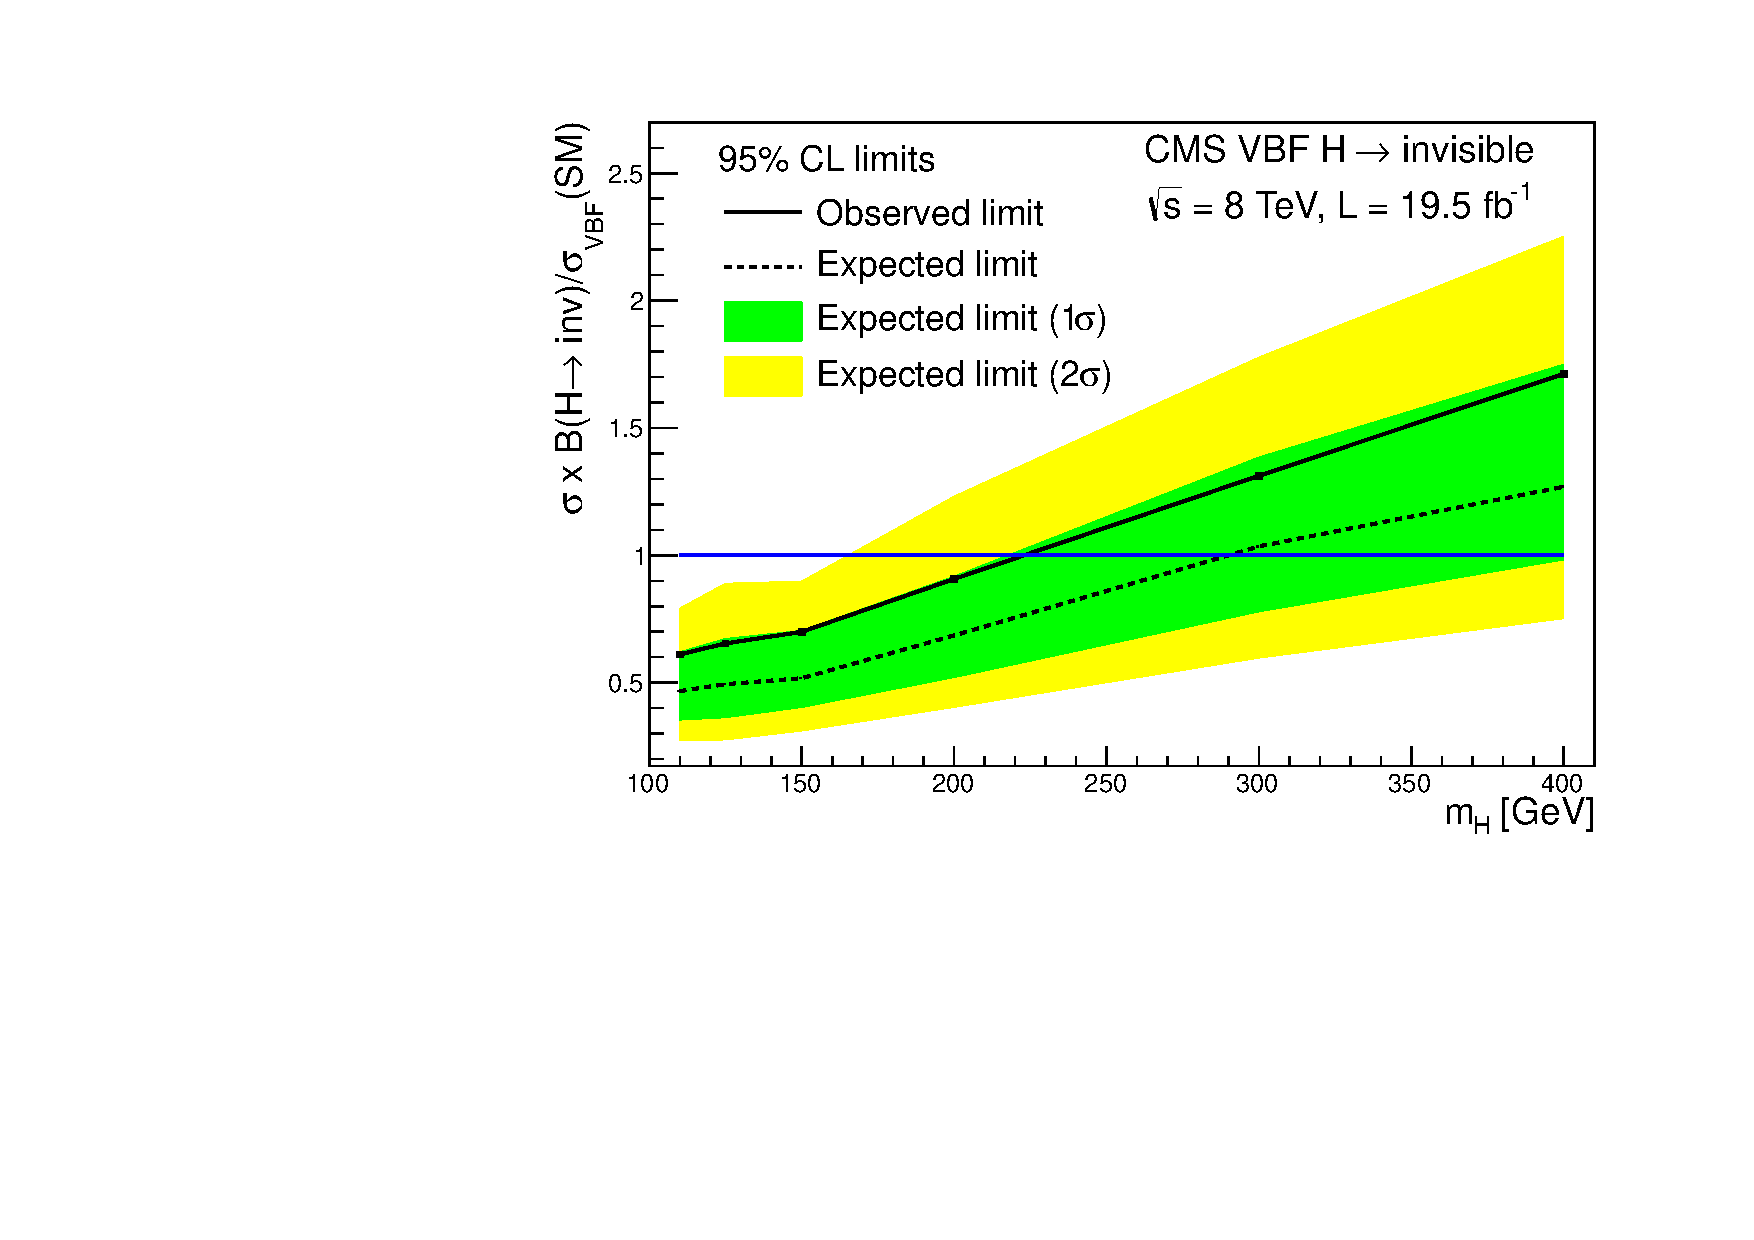
\includegraphics[width=0.49\textwidth]{Images/VBF-Limit.pdf}}
  \caption{}%!!REDO CAPTION
  \label{vbflimits}
\end{figure}

\begin{figure}
  \centering
  \raisebox{-0.5\height}{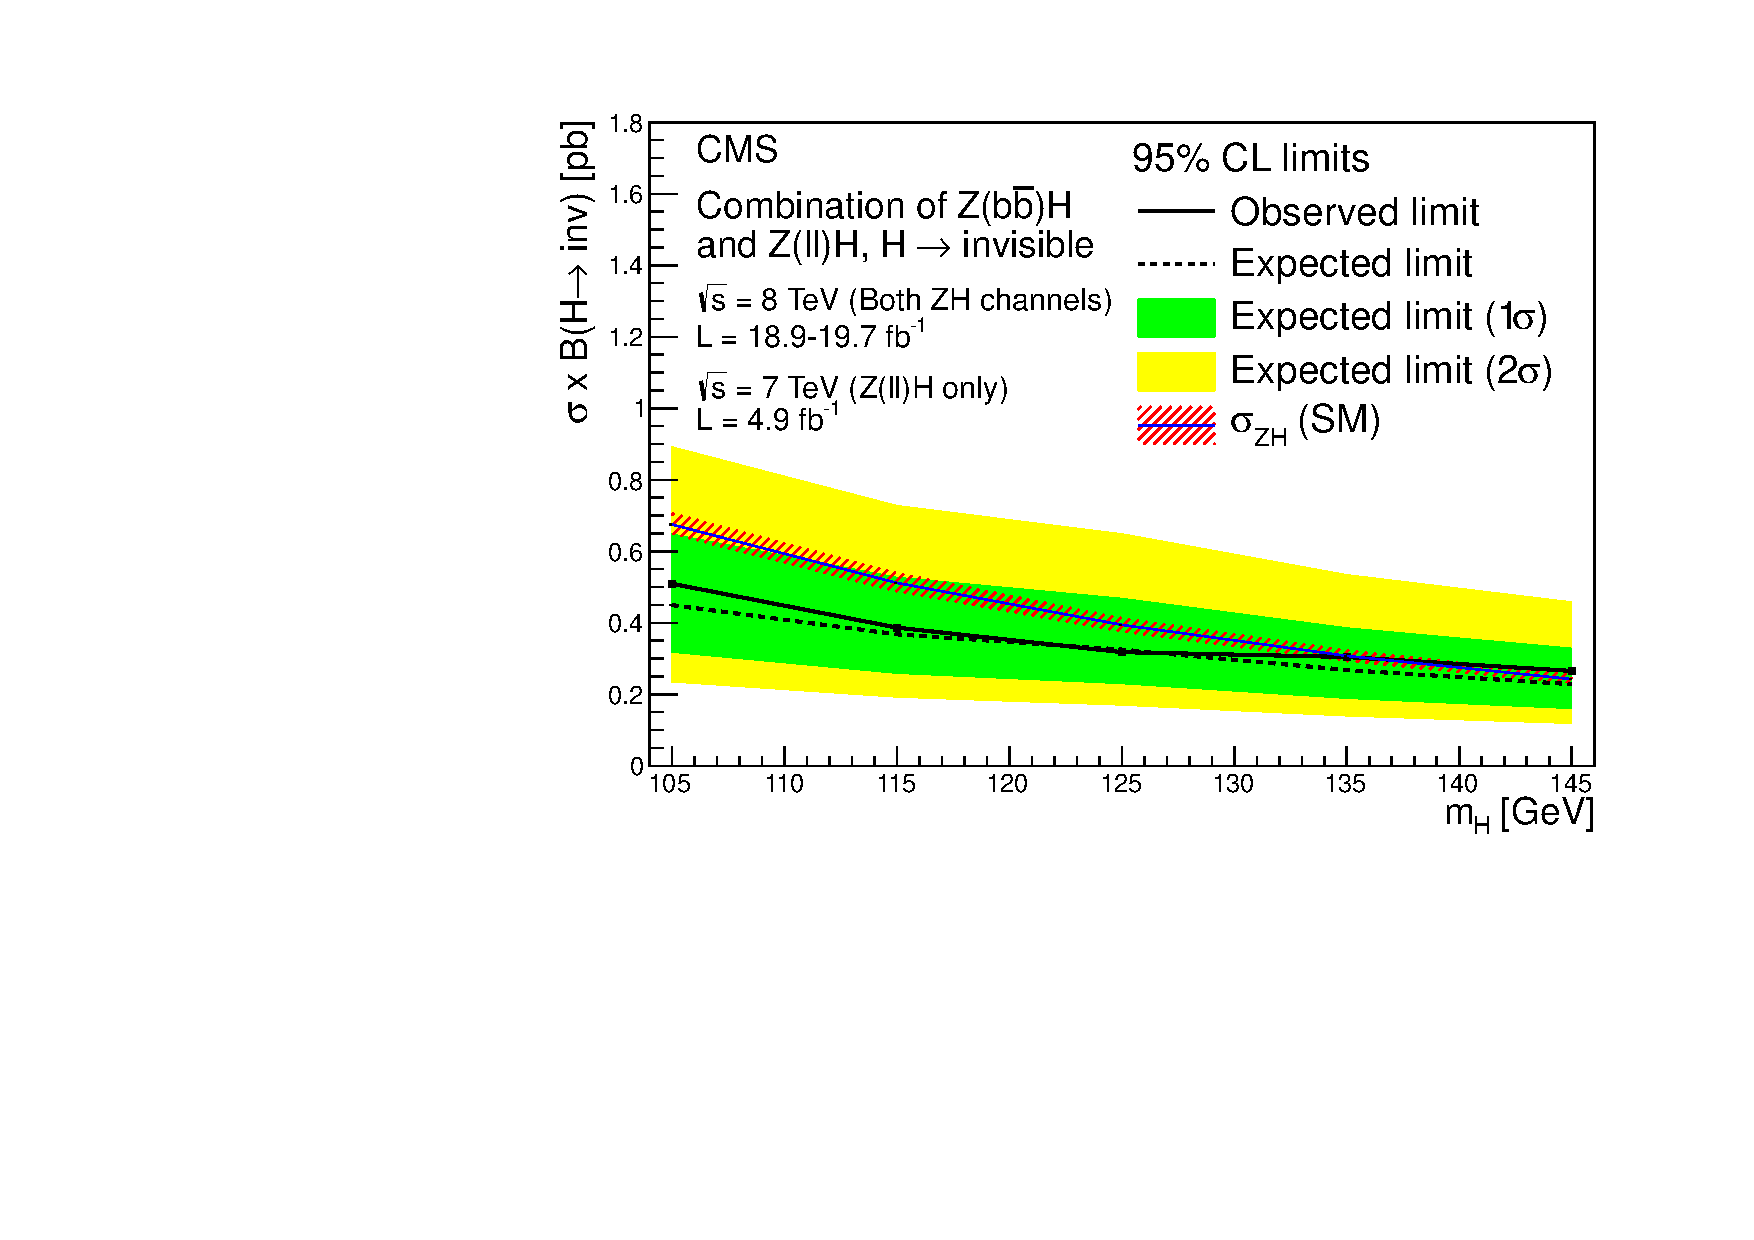
\includegraphics[width=0.49\textwidth]{Images/ZH-XSLimit.pdf}}
  \raisebox{-0.5\height}{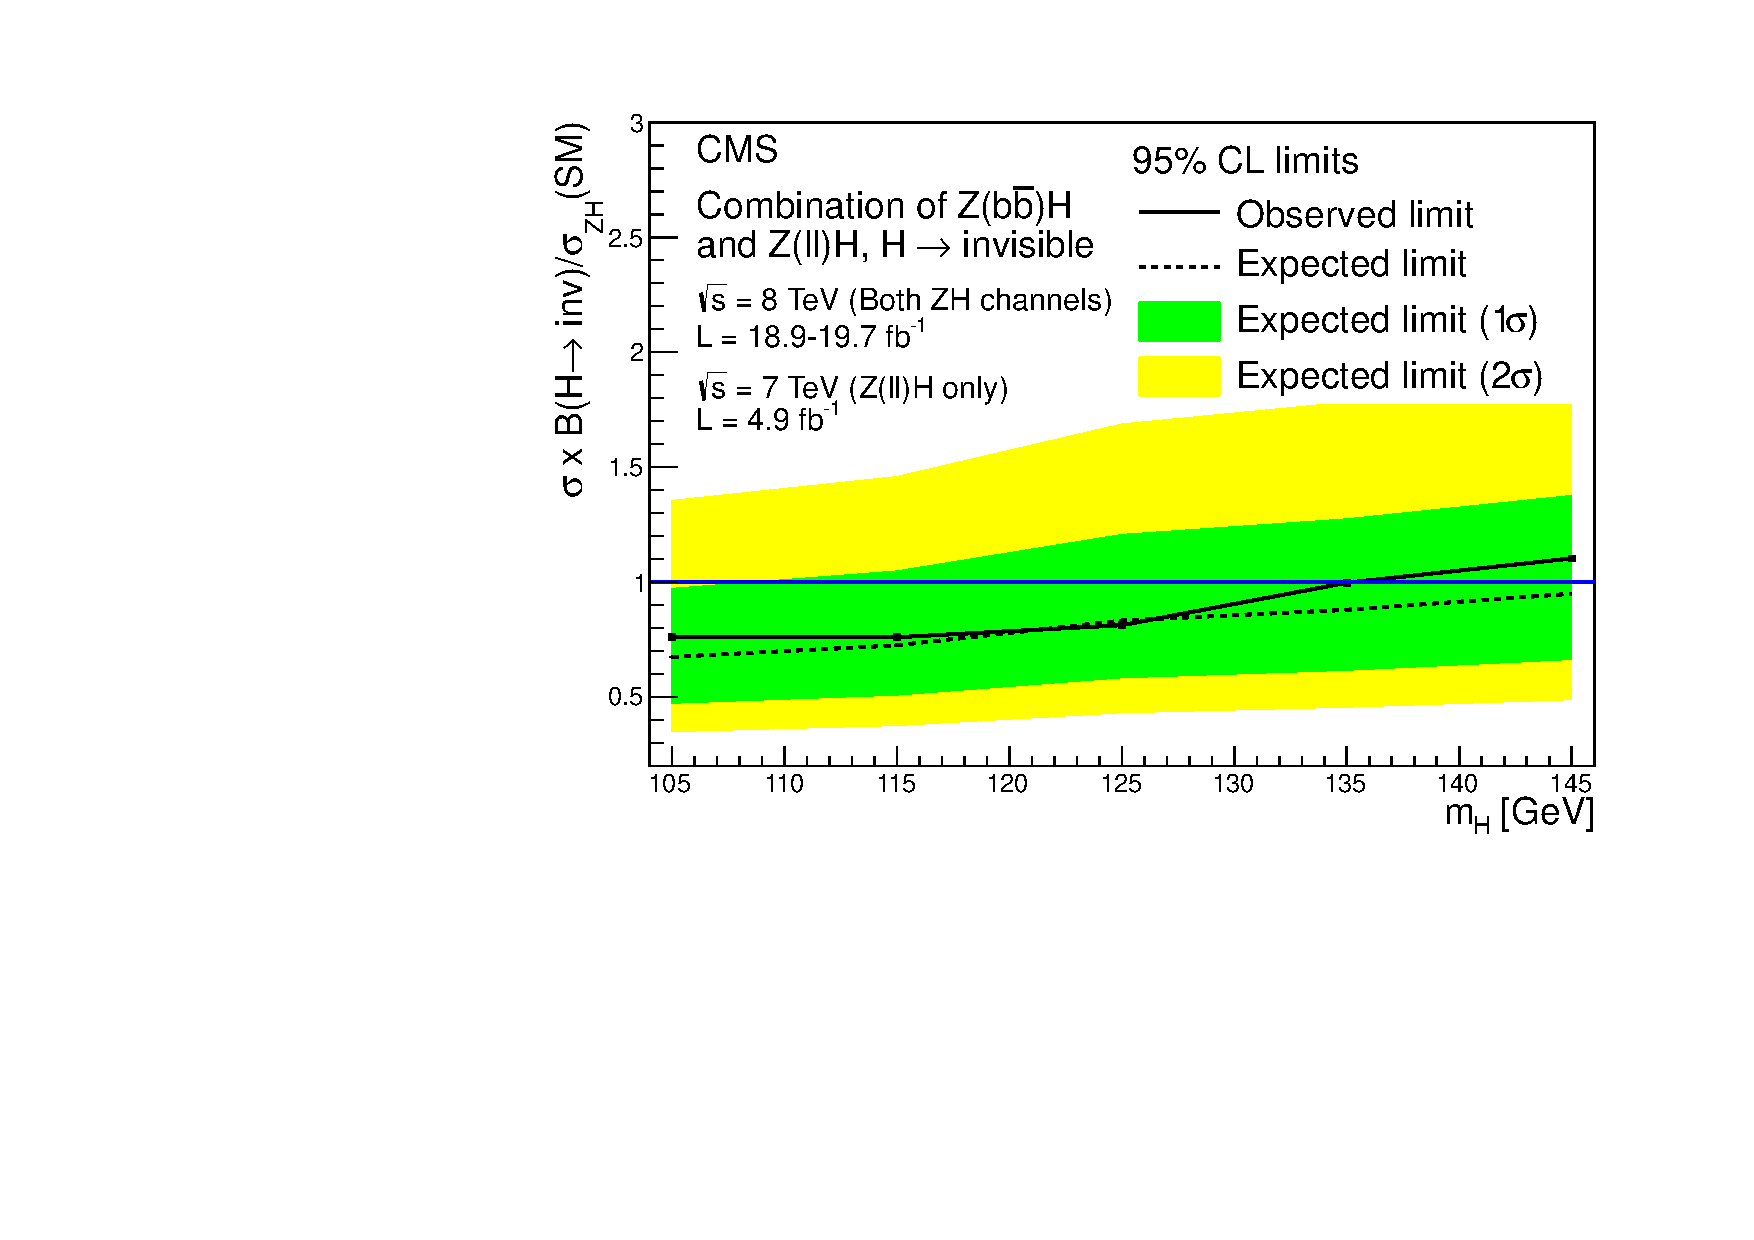
\includegraphics[width=0.49\textwidth]{Images/ZH-Limit.pdf}}
  \caption{}%!!REDO CAPTION
  \label{zhlimits}
\end{figure}

\begin{figure}
  \centering
  \raisebox{-0.5\height}{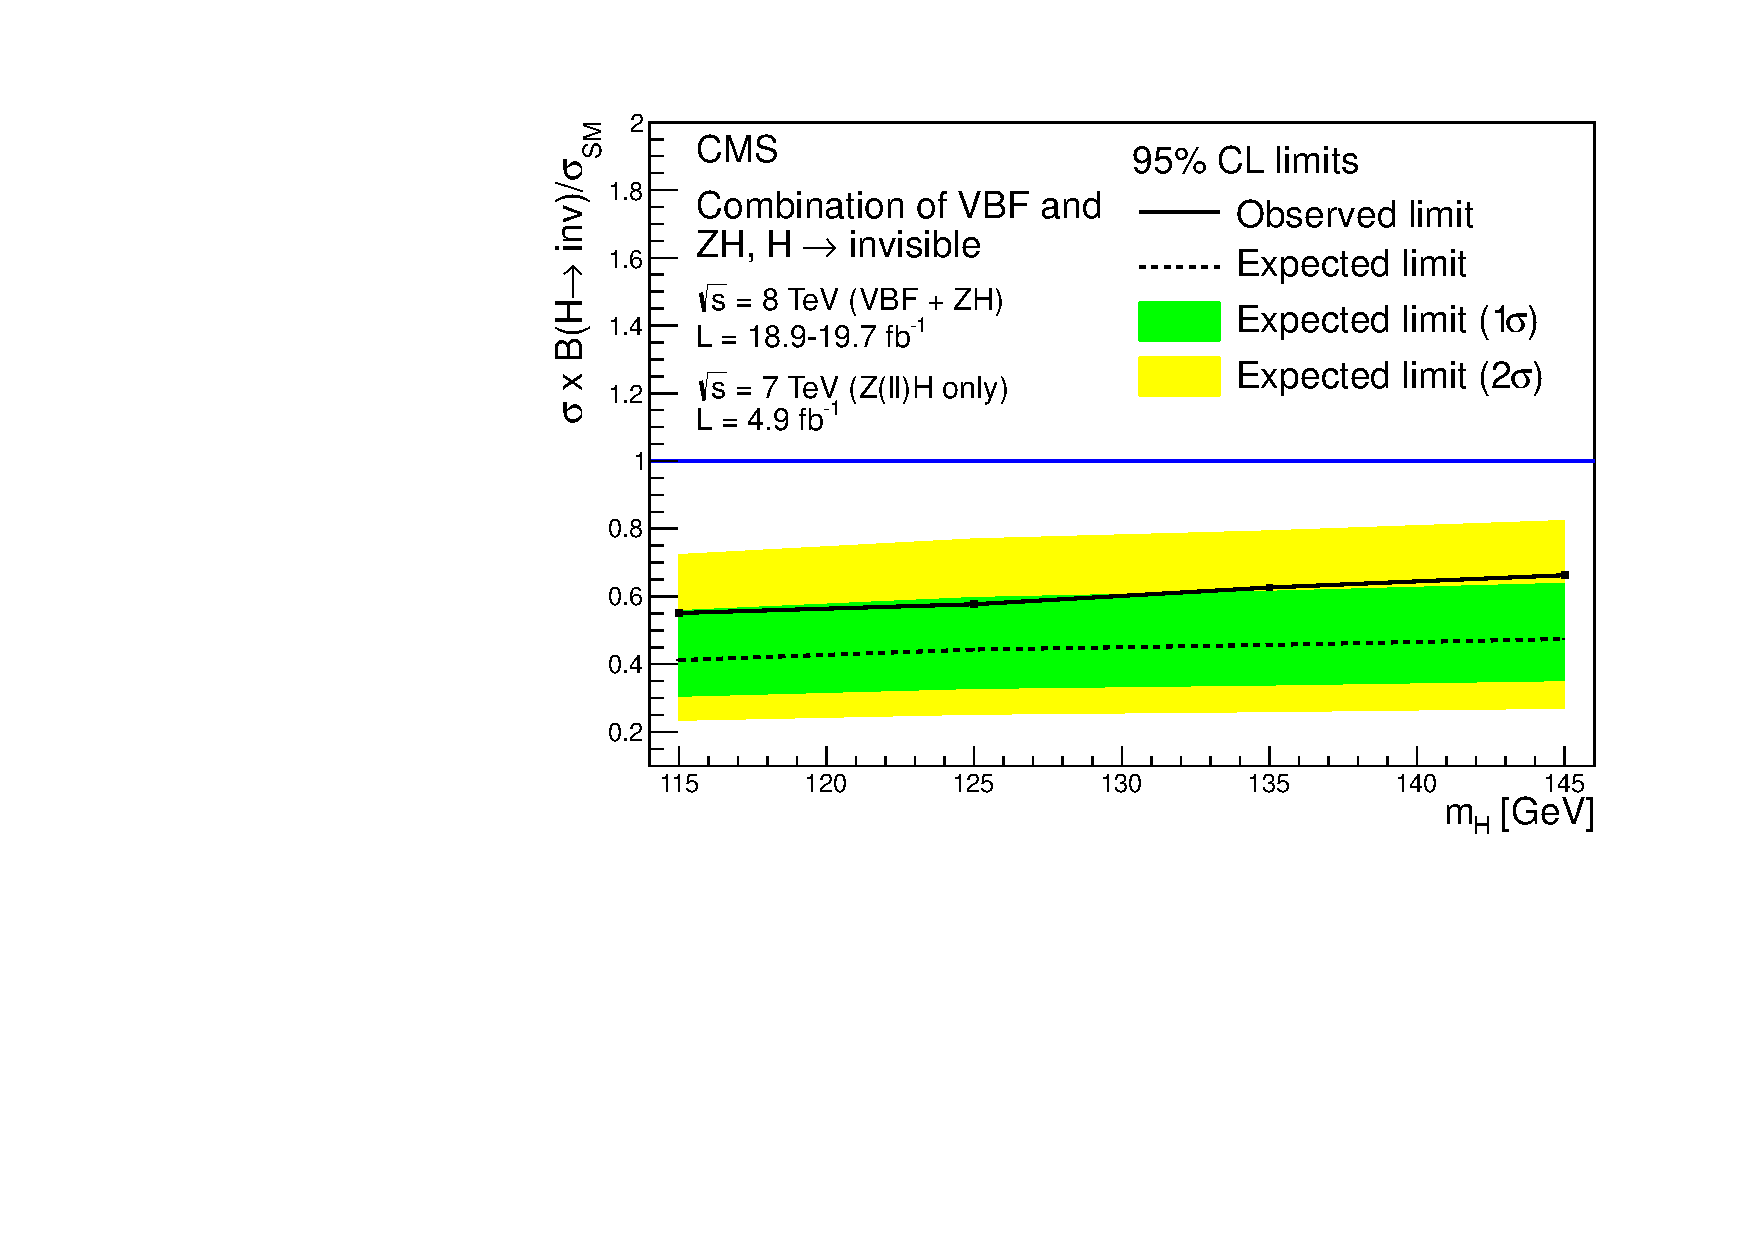
\includegraphics[width=0.49\textwidth]{Images/Combination-Limit.pdf}}
  \raisebox{-0.5\height}{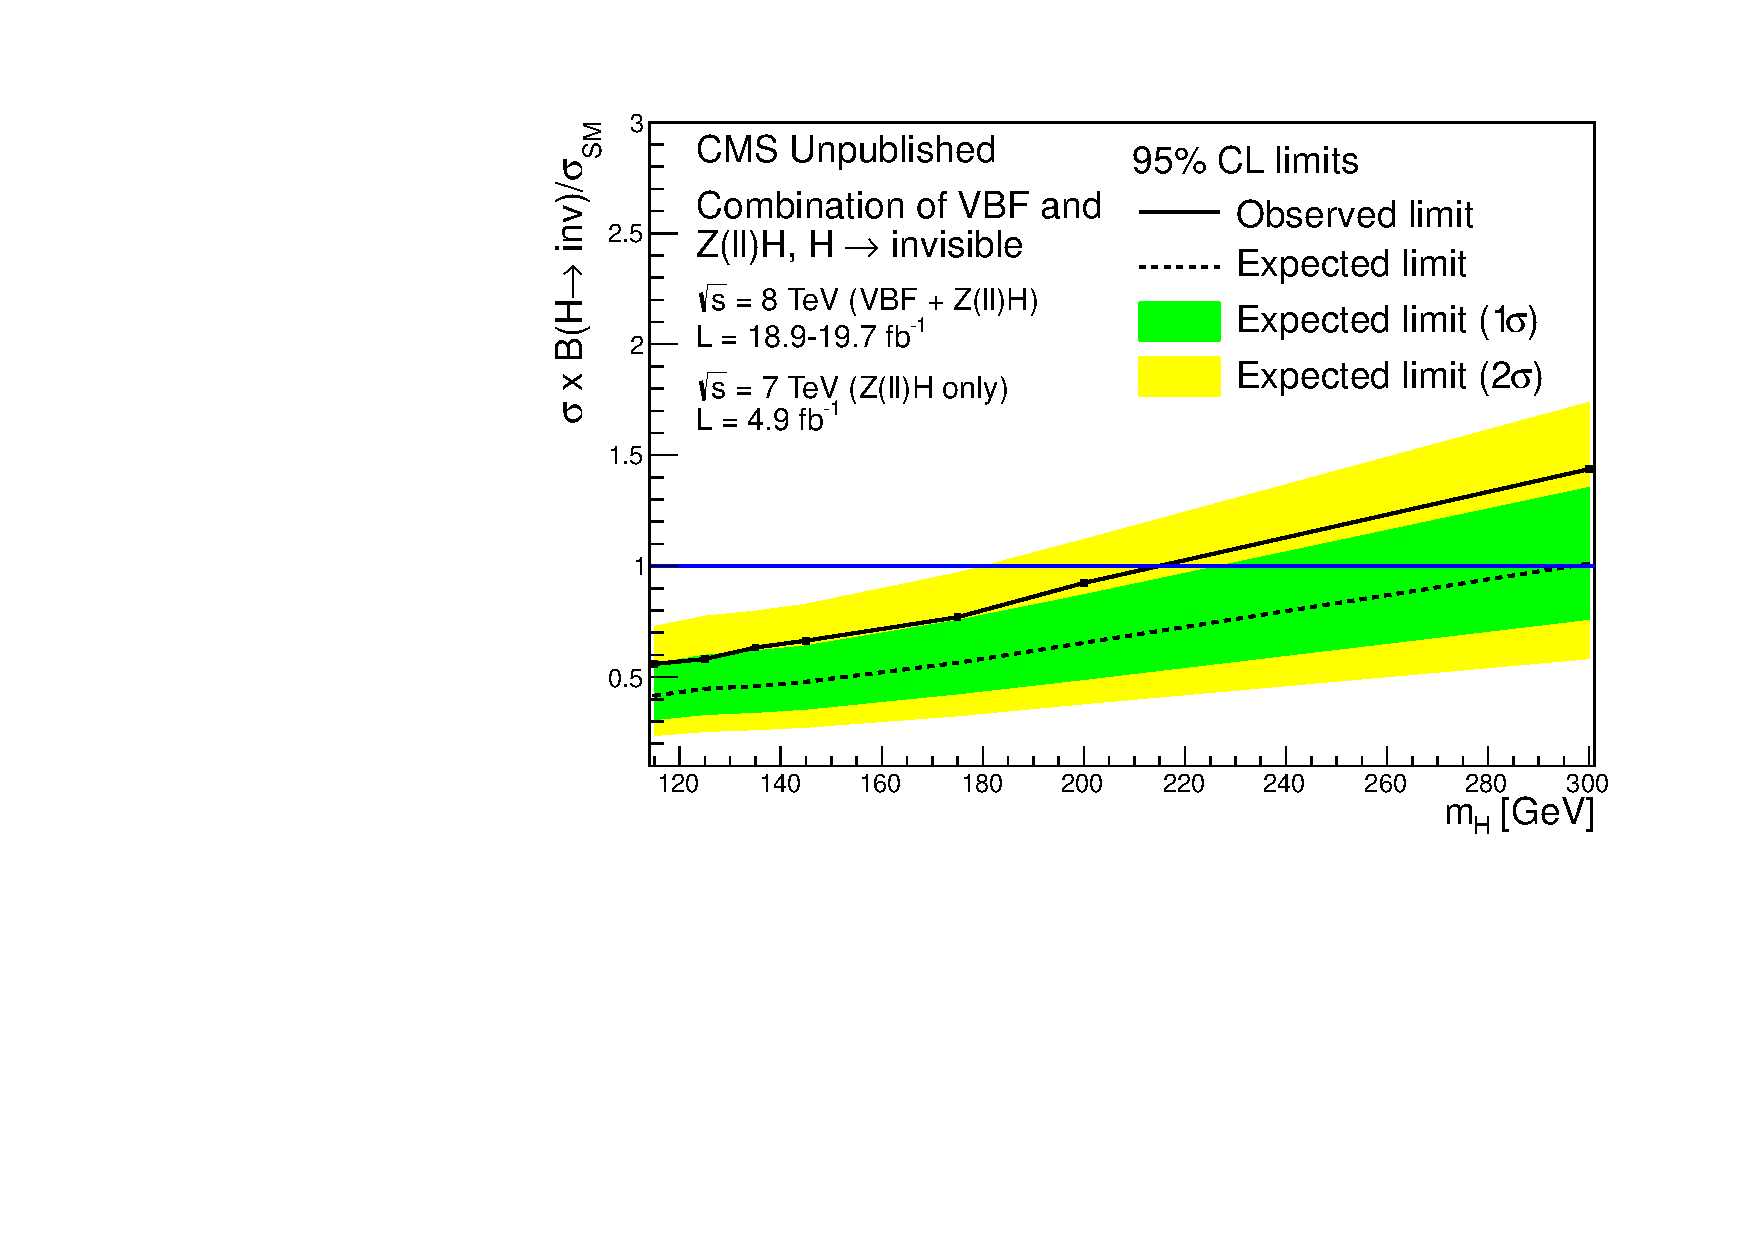
\includegraphics[width=0.49\textwidth]{Images/VBF-ZllH-HighMassLimit.pdf}}
  \caption{}%!!REDO CAPTION
  \label{combinedlimits}
\end{figure}


\section{Future work}
My thesis will focus on searches for Higgs boson decays to invisible final states, particularly those in the VBF channel and the combination of results between channels. I have begun by participating in the analysis of the CMS prompt 2012 data for the VBF channel Higgs to invisible search and performing the combination between the VBF and the two ZH channels. I will now move on to using the parked data, discussed in section \ref{cmslhc} from 2012 to update the VBF Higgs to invisible search; this is of particular importance as the LHC is shut down as of mid-February 2013 for two years, so the parked data is the only available unanalysed data. 

Depending on the outcome of this work I will study preparations for analyses after the LHC restarts. I will also perform service work, which is required for continuing authorship in the CMS Collaboration, this will involve working on the computing or calorimetry upgrade of CMS.


\begin{thebibliography}{999}
%!!UPDATE REALLY NEEDS AN OVERHAUL
\bibitem{glashow}S. Glashow, ``Partial-symmetries of weak interactions'', Nucl. Phys. 22 (1961) 579.
\bibitem{weinberg}S. Weinberg, ``A Model of Leptons'', Phys. Rev. lett. 19 (1967) 1264.
\bibitem{salam}A. Salam, ``Weak and electromagnetic interactions,'', in: N. Svartholm (Ed.), Elementary Particle Physics: Relativistic Groups and Analyticity, Prodeedings of the Eighth Nobel Symposium, Almquvist and Wiskell, 1968, p. 367.
\bibitem{wdiscovery} UA1 Collaboration, ``Experimental observation of isolated large transverse energy electrons with associated missing energy at $\sqrt{s} = 540\,\rm{GeV}$,'' Phys. Lett. B122 (1983) 103. 
\bibitem{zdiscovery} UA1 Collaboration,  ``Experimental Observation of Lepton Pairs of Invariant Mass Around 95 GeV at the CERN SPS Collider'', Phys. Lett. B126 (1983) 398. 
\bibitem{englertbrout} F. Englert, R. Brout, ``Broken Symmetry and the Mass of Gauge Vector Mesons'', Phys. Rev. Lett. 13 (1964) 321.
\bibitem{higgs1} P.W. Higgs, ``Broken symmetries, massless particles and gauge fields'', Phys. Lett. 12 (1964) 132.
\bibitem{higgs2} P.W. Higgs, ``Broken Symmetries and the Masses of Gauge Bosons'', Phys. Rev. lett. 13 (1964) 508.
\bibitem{guralniketc} G. Guralnik, C. Hagen, T.W.B. Kibble, ``Global Conservation Laws and Massless Particles'', Phys. Rev. Lett. 13 (1964) 585.
\bibitem{higgs3} P.W. Higgs, ``Spontaneous Symmetry Breakdown without Massless Bosons'', Phys. Rev. 145 (1966) 1156.
\bibitem{kibble} T.W.B. Kibble, ``Symmetry breaking in non-Abelian gauge theories'', Phys. Rev. 155 (1967) 1554.
\bibitem{atlasdiscovery} ATLAS Collaboration, ``Observation of a new particle in the search for the Standard Model Higgs boson with the ATLAS detector at the LHC'', Phys. Lett. B716 (2012) 1.
\bibitem{cmsdiscovery} CMS Collaboration, ``Observation of a new boson at a mass of 125 GeV with the CMS experiment at the LHC'', Phys. Lett. B 716 (2012) 30.
\bibitem{lhc} L. Evans, P. Bryant (Eds.), ``LHC Machine'', JInst. 3 (2008) S08001.
\bibitem{cmstdr} CMS Collaboration, ``The CMS experiment at the CERN LHC'', JInst. 3 (2008) S08004.
\bibitem{hcalres} CMS HCAL Collaboration, ``Energy Response and Longitudinal Shower Profiles Measured in CMS HCAL and Comparison with GEANT4'', CMS NOTE 2006/143.
\bibitem{higgworkgroup2001} Girolamo et al, ``The Higgs Working Group: Summary report, C. Experimental Observation of an invisible Higgs Boson at LHC'', arXiv:hep-ph/0203056 (2001).
\bibitem{parkeddata} CMS Collaboration, Data Parking and Data Scouting at the CMS Experiment, CMS-DP-2012-022.
\bibitem{bds} Y. Bai et al, ``Measuring the Invisible Higgs Width at the 7 and 8 TeV LHC'', arXiv:1112.4496.
\bibitem{zeppenfeld} D. Zeppenfeld, ``Observing an invisible Higgs boson'', Phys. Lett. B 495 (2000) 147.
\bibitem{hig1330} CMS Collaboration, ``Search for invisible decays of Higgs bosons in the vector boson fusion and associated ZH production modes'', arxiv:1404.1344 [hep-ex].
\bibitem{lhchxswg} LHC Higgs Cross Section Working Group, S.~Dittmaier, C.~Mariotti, G.~Passarino, and R.~Tanaka (Eds.), 
  {\sl Handbook of LHC Higgs Cross Sections: 2. Differential Distributions}, 
  CERN-2012-002 (CERN, Geneva, 2012), {\tt arXiv:1201.3084 [hep-ph]}.
\bibitem{hcpcomb2012} CMS Collaboration, ``Combination of standard model Higgs boson searches and measurements of the properties of a new boson with a mass near 125 GeV'', CMS PAS HIG-12-045 (2012).
\bibitem{comb2011} CMS Collaboration, ''Combined results of searches for the standard model Higgs boson in pp collisions at $\sqrt{s} = 7 \,\rm{TeV}$'', Phys. Lett. B 710 (2012) 26.
\bibitem{lhccomb1} ATLAS and CMS Collaborations, LHC Higgs Combination Group, ``Procedure for the LHC Higgs bonson search combination in Summer 2011'', CMS NOTE 2011/005.


\end{thebibliography}

\end{fmffile}
\end{document}
